\chapter{Introduction}
\label{introchap}
\section{To Do:}
\begin{itemize}
    \item make sure there are hard-coded spaces (or smarter ways of doing that) after all instances of \textbackslash IRL, \textbackslash degdip, or any other macros you made.
    \item replace all the ind varb, dep varb, ling varb (and relevant lemmas) stuff with better, less confusing terminology (noticed re: ch 5).
    \item come up with a better term than ``generalization'' since it's not actually dependent on what they did in the shadowing block.
    \item take care of all the highlighted bits.
    \item decide whether ``mandarinization'' (and its lemmas) should be capitalized or not, and make it consistent throughout the dissertation. Also, check that it's spelled properly everywhere, cuz it's not in overleaf's dictionary.
    \item decide what your dep varbs, ind varbs, and ling varbs should be called (including whether they should be capitalized) and make sure your terminology is consistent throughout. Right now I think the variables themselves should be capitalized; ``Age'' would be the thing that predicts generalization, but ``age'' is a factor that's commonly cited as having an effect on participation in sound change (or whatever).
    \item deal with the fact that flipping the signs means different things for different variables in Ch 5.
    \item come up with better terminology to describe the predictors you use (BLP, IAT, etc.). ``Socio-psychological'' feels particularly wishy-washy.
    \item check for and standardize hyphenation of\begin{enumerate}
        \item ``pre-'' and ``post-test''
        \item ``hyper-standard''
        \item ``intra-'' and ``inter-personal''
    \end{enumerate}
\end{itemize}

\section{Important bits of theory}
\label{sec:theory}
\subsection{Trudgill}
One important bit of theory is Trudgill's (1986) theory about how mutually-intelligible dialects change when they come into contact with one another. The core idea (for the purpose of this dissertation) is that when two groups of people who speak different dialects interact over time, they undergo the following process:
\begin{enumerate}
\item Short-term accommodation
\item Long-term accommodation
\item Dialect change
\end{enumerate}
I'm going to describe what these mean now!

So what Trudgill means by short-term accommodation is what is often referred to sort of generally in the \hl{socio-psychological} literature as "interactional synchrony." It's the process by which interlocutors come to generally behave--and more specifically, speak--like each other. So, for example, if I were speaking with Donald Trump Sr., I might start using grandiose terminology, or short, repetitive sentences (FIND CITATION ABOUT HOW TRUMP SPEAKS), mirroring elements of his syntax, word choice, and phonology, in addition to mimicking elements of his body posture.

Long-term accommodation is when an individual has been speaking with someone else for long enough and frequently enough that they hold on to the features of their interlocutor's speech that they've picked up through short-term accommodation. That is, even after I'm no longer speaking to Donald Trump, I continue to use that same grandiose terminology, phonology, or posture.

Dialect change, then, is what happens once I've taken these features of Mr. Trump's behavior, and carried them back to my home speech community. If after returning to my home town I continue to speak the way Mr. Trump does, it is possible that features of my speech that I have adopted from my encounter with Mr. Trump will then spread to other members of my community as I interact with them and they engage in acts of short-term accommodation with me. (This isn't really the idea, I think, of Trudgill's third step. The third step is actually maybe more just like when enough people have completed the second step, you can be like ``Look! The dialect has changed!'' but I'm not so concerned with that part of the problem.)

The interesting thing here is that, as observed by \citet{auer2005role} ``[i]t [is] difficult[...]to find evidence for the co-occurrence of interpersonal accommodation and community-level change.'' The issue I'm trying to address with this dissertation is that there doesn't really seem to be any research that looks at whether individuals actually engage in long-term accommodation. So, I've tried to design an experiment that would function as empirical evidence that long-term accommodation is a thing. (I should add something about the persistence hypothesis. Look at Sonderegger 2012 again and pull out any citations he has that indicate that short-term imitation can persist into the future even days after an initial interaction. \cite{goldinger2000role}, for example, says that listeners perceive speakers as being more similar to a recording that the speaker listened to a week earlier (I think), so like the speaker listened, imitated, and then a week later was still imitate-y sounding.) 

What was the other theoretical stuff I thought was interesting a few weeks ago? Shit, I should have like written it on a scrap of paper or something. Maybe it had something to do with the framing I came up with for my LSA abstract. I'm gonna look at that now real quick.

\subsection{Sonderegger}
So, Sonderegger (2012) makes some important points about the fact that for there to be change over time, change in the moment must \textit{persist}. He talks about the ``persistence hypothesis.'' This hypothesis basically says ``that short-term shifts which an individual makes during interaction can and do accumulate over time into long-term change'' \citep[p.102]{sonderegger2012phonetic}. Sonderegger finds support for a weakish form of the persistence hypothesis.

\section{Background on the IRL dialect situation}
Nanjing, China’s ``southern capital,'' is a mid-sized Chinese city, population roughly 8.2 million. Like many cities in China, Nanjing’s distinct local dialect is undergoing marked contact-induced language change \citep{bao1980sixty}. For the last several hundred years, Nanjing Dialect has been gradually absorbing features of more prestigious northern speech varieties, with change being particularly rapid over the last several decades thanks to a national policy of promoting PTH as the language of media, education, and business. While most of the questions that I am trying to answer in this dissertation are not specific to the situation in Nanjing, Nanjing does provide a valuable case study for looking at how language contact may lead to sound change.

In this section, I plan to expand upon the comments I’ve already made with respect to the nature of face-to-face interaction in Nanjing, and particularly to describe the nature of the diglossic situation that exists there today, relying on my interview data and the self-reported behavior of my speakers. There is also at least one source that deals with the subject of code choice in Nanjing \citep{xu2006nanjing}.



\pagebreak
THIS PAGE INTENTIONALLY LEFT BLANK
\pagebreak

THIS IS BOILERPLATE THAT THE GRAD SCHOOL ADDED
This sample document illustrates how to use the
{\tt thesis} class, originally written by John P. Weiss.
Some requirements of the Graduate School are written
into that file; page size, line spacing, appropriate
placement of captions for tables and figures, etc.
Revisions by Hongcheng Ni make it possible to use the
(optional)
\verb2\usepackage{hyperref}2 command to enable
internal hyperlinks in the final PDF document.
Other tasks of conforming to the requirements are
left to other existing \LaTeX{} packages.
For example, a common problem is to insert graphics ---
figures and tables --- into the body of the thesis.  For
this one should use the {\tt graphicx} package, which is
part of the standard \TeX{} distribution.  Likewise, the
Grad School specs say that a large table may be displayed
in landscape mode at reduced size, but its caption must
also be in rotated position, in the same font and size as
the normal text in the body of the thesis.  To accomplish
this, the user must invoke the {\tt rotating} package,
available online.


Figure \ref{xfigDiagram} shows an image from a PDF file
imported into this document
using the \verb2graphicx2 package.
The command \verb2\usepackage{graphicx}2, which appears
near the very top of the main \LaTeX{} file, reads in
this package which defines the
\verb2\includegraphics{}2 macro.


\begin{figure}[htbp]
	\caption[Cylinder and measurements]{
	This diagram of a cylinder and various
	measurements and quantities was actually
	made using {\bf xfig}, a freeware
	drawing program for Unix systems.
	Diagrams can be exported directly to PDF
	files, the preferred format for
	vector graphics.  Vector graphics can
	be magnified indefinitely without degradation,
	whereas bitmap images (JPG and PNG)
	must be pretty high-resolution if you don't
	want them looking all pixellated when
	magnified.
	}
    \begin{center}
	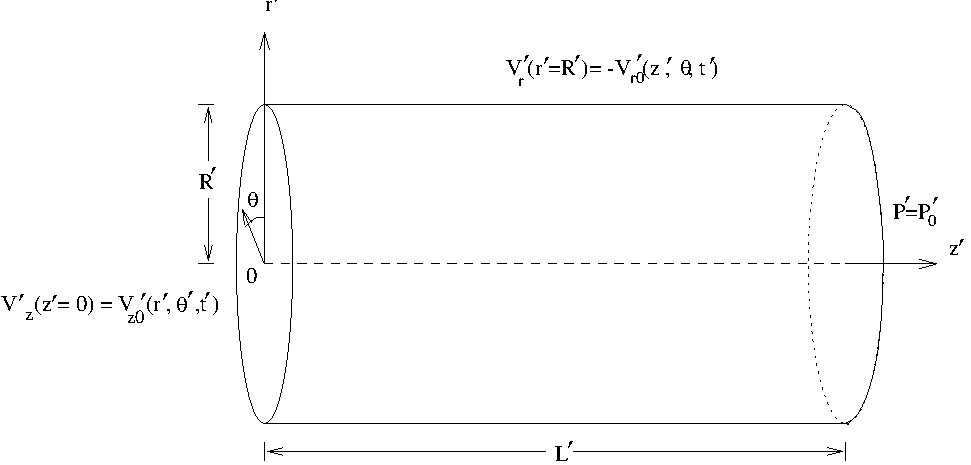
\includegraphics[width=100mm]{figs/cyl.pdf}
    \end{center}
\label{xfigDiagram}
\end{figure}


\begin{figure}[htbp]
    \caption[Bitmap images]{
	The JPEG bitmap format is great for photos but
	crummy for diagrams (including drawings, graphs,
	charts) because it can't gracefully handle sharp edges.
	Note the same bitmap image below from a PNG file and
	from a JPG file; the latter shows characteristic
	``ringing'' at sharp edges -- including text!
	Seriously, magnify and look closely at the JPG's
	awful lines and edges.
	Vector-format PDF is the best for diagrams, but
	if you must use a bitmap image, let it be PNG.
	~ (Left: file {\it drawing.png}.
	Right: file {\it drawing.jpg}.)
	}
    \begin{center}
	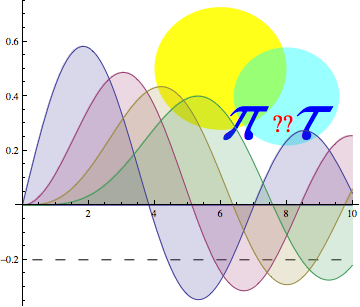
\includegraphics[width=70mm]{figs/drawing.png}
	${}^{}$ ~
	${}^{}$ ~
	${}^{}$
	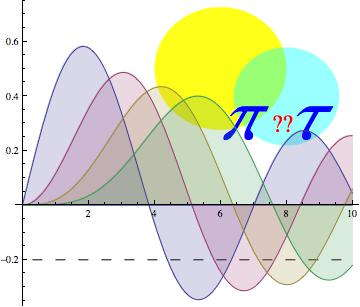
\includegraphics[width=70mm]{figs/drawing.jpg}
    \end{center}
\label{bitmapImages}
\end{figure}



\section{Lists in {\tt thesis} class}

In {\tt thesis} class (for Colorado University),
lists are defined so that nested lists will be
numbered or marked appropriately.
First, an itemized (non-enumerated) list
prefaces each item with a bullet.
Nested itemized list use asterisks,
then dashes, then dots.
These lists are typed between
the \verb2\begin{itemize}2
and \verb2\end{itemize}2
commands.

\begin{itemize}
  \item{} This is ``itemized'' item A.
  \item{} This is ``itemized'' item B.
  \item{} This is ``itemized'' item C.
  \begin{itemize}
    \item{} This is ``itemized'' subitem A.
    \begin{itemize}
      \item{} This is ``itemized'' subsubitem A.
      \begin{itemize}
        \item{} This is ``itemized'' subsubsubitem A.
      \end{itemize}
      \item{} This is ``itemized'' subsubitem B.
    \end{itemize}
    \item{} This is ``itemized'' subitem B.
  \end{itemize}
  \item{} This is ``itemized'' item D.
\end{itemize}

Enumerated lists use the commands
\verb2\begin{enumerate}2 and
\verb2\end{enumerate}2,
and nested enumerations appear like this.

\begin{enumerate}
  \item{} This is ``enumerated'' item A.
  \item{} This is ``enumerated'' item B.
  \item{} This is ``enumerated'' item C.
  \begin{enumerate}
    \item{} This is ``enumerated'' subitem A.
    \begin{enumerate}
      \item{} This is ``enumerated'' subsubitem A.
      \begin{enumerate}
        \item{} This is ``enumerated'' subsubsubitem A.
      \end{enumerate}
      \item{} This is ``enumerated'' subsubitem B.
    \end{enumerate}
    \item{} This is ``enumerated'' subitem B.
  \end{enumerate}
  \item{} This is ``enumerated'' item D.
\end{enumerate}


The work presented
here\footnote{Footnotes are handled neatly by \LaTeX.}
is an extension of Lao\cite{lao:thesis}
and Lao et~al.\cite{lao:paper},
fictional references that are in the bibliographic
source file \verb9refs.bib9.

\begin{table}[htb]
    \caption[Example of a table with its own footnotes]{
	Here is an example of a table with its own footnotes.
	Don't use the $\backslash${\tt footnote} macro if you
	don't want the footnotes at the bottom of the page.
	Also, note that in a thesis the caption goes
	\emph{above} a table, unlike figures.
	}
    \begin{center}
    \begin{tabular}{||l|c|c|c|c||} \hline
	& $S$ & $P$ &   $Q^{\ast}$  & $D^{\dagger}$ \\	% footnote symbols!
	wave form & (kVA) & (kW) & (kVAr) & (kVAd) \\  \hline \hline
	Fig.  \ref{xfigDiagram}a  & 25.48 & 25.00 & -2.82 & 4.03 \\ \hline
	Fig.  \ref{xfigDiagram}b  & 25.11 & 18.02 & -9.75 & 14.52 \\ \hline
	Table \ref{pdftable}  & 24.98 & 22.26 & 9.19 & 6.64 \\ \hline
	Table \ref{powertable}  & 23.48 & 15.00 & 6.59 & 16.82 \\ \hline
	Fig.  \ref{pyramid}  & 24.64 & 22.81 & -0.44 & 9.3 \\ \hline
	\end{tabular}
   \\ \rule{0mm}{5mm}
   ${}^\ast$kVAr means reactive power.		% footnote symbol
\\ ${}^\dagger$kVAd means distortion power.	% footnote symbol
\end{center}
\label{powertable}
\end{table}


